\documentclass[13pt,oneside]{book}
\usepackage[utf8]{inputenc}
\usepackage{url}
\usepackage{listings}
\usepackage{graphicx}

\usepackage{geometry}
\geometry{a4paper, left=20mm, right=20mm, top=20mm, bottom=20mm}
\usepackage[margin=1.2in]{geometry}
\usepackage[toc,page]{appendix}
\usepackage{graphicx}
\usepackage{natbib}
\usepackage{lipsum}
\usepackage{caption}

\begin{document}

\captionsetup[figure]{margin=1.5cm,font=small,labelfont={bf},name={Figure},labelsep=colon,textfont={it}}
\captionsetup[table]{margin=1.5cm,font=small,labelfont={bf},name={Table},labelsep=colon,textfont={it}}
\setlipsumdefault{1}

\begin{titlepage}
\begin{center}
{\LARGE College Of Engineering Trivandrum}\\[3cm]
\linespread{1.2}\huge {\bfseries System Software Lab}\\[3cm]
\linespread{1}

\includegraphics[width=5cm]{img/emblem.jpeg}\\[3cm]
{\Large GOKUL K\\ S5  CSE \\ Roll No:21\\ TVE18CS021 }\\[1cm]


\textit{ }\\[2cm]
Department of Computer Science\\[0.2cm]
\today
\end{center}

\end{titlepage}

\newpage

\begin{frame}{}
    \centering
    \hspace*{-0.5cm}
    $\vcenter{\hbox{
\includegraphics[width=1.5cm]{img/emblem.jpeg}}}$
    $\vcenter{\resizebox{0.95\textwidth}{!}{
        \begin{tabular}{c}
             CS331 - System Software Lab $\cdot$ 2020 $\cdot$   \\
             \hline 
        \end{tabular}
    }}$
\end{frame}
\section*{Cycle 1}
\section*{Expt 5}
\begin{center}
    \Large{Symbol Table Hashing}
\end{center}
\section*{Aim}
\large
To implement symbol table with hashing

\section*{Algorithm} 
    \begin{verbatim}
1 Start .
2 Define the structure of the Symbol Table
3 Enter the choice for performing the operations in the Symbol Table
4 If the entered choice is 1 , search the symbol table for the symbol
to be
5 inserted . If the symbol is already present , it displays "
Duplicate Symbol ",
6 else , insert the symbol and the corresponding address in the symbol
table .
7 If the entered choice is 2 , delete the particular symbol .
8 If the entered choice is 3 , the symbols present in the symbol table
are
9 displayed .
10 If the entered choice is 4 , the symbol is searched in the symbol
table . If it
11 is not found in the symbol table it displays "Not found ".
12 If the entered choice is 5 , the symbol to be modified is searched
in the
13 symbol table . The address of the label can be modified .
14 Enter choice 6 to exit the program .
15 Stop
	\end{verbatim}

\section*{Source Code}
\small

\begin{lstlisting}[language=C]
	#include <stdio.h>
	#include <stdlib.h>
	#include <string.h>
	
	#define SIZE 20
	
	struct SymTabItem
	{
		char label[10];
		char datatype[10];
		int address;
	
		struct SymTabItem * next;
	};
	
	struct SymTabItem * hash_map[SIZE];
	
	struct SymTabItem * create_item(char label[], char datatype[], int address)
	{
		struct SymTabItem * item;
		item = malloc(sizeof(struct SymTabItem));
		item->address = address;
		strcpy(item->datatype, datatype);
		strcpy(item->label, label);
		item->next = NULL;
	
		return item;
	}
	
	// Hash function presented in K&R version 2
	unsigned calculate_hash(char *s)
	{
		unsigned hashval;
	
		for (hashval = 0; *s != '\0'; s++)
			hashval = *s + 31 * hashval;
	
		return hashval % SIZE;
	}
	
	void insert(char label[], char datatype[], int address)
	{
		unsigned hash = calculate_hash(label);
		struct SymTabItem * curr_item;
		struct SymTabItem * iter = hash_map[hash];
	
		if(iter == NULL)
		{
			hash_map[hash] = create_item(label, datatype, address);
			printf("Insertion successful\n");
			return;
		}
	
		while(iter->next != NULL)
		{
			if(strcmp(iter->label, label) == 0)
			{
				printf("Duplicate symbol\n");
				return;
			}
	
			iter = iter->next;
		}
	
		iter->next = create_item(label, datatype, address);
	}
	
	void delete(char label[])
	{
		unsigned hash = calculate_hash(label);
		struct SymTabItem * prev, * iter;
		prev = iter = hash_map[hash];
	
		while(iter != NULL)
		{
			if(strcmp(iter->label, label) == 0)
			{
				// If the first element is the label
				if(prev == iter) hash_map[hash] = NULL;
				else prev->next = iter->next;
	
				printf("Deleted succesfully\n");
				free(iter);
				return;	
			}
	
			prev = iter;
			iter = iter->next;
		}
	
		printf("No such label present\n");
		return;
	}
	
	void display()
	{
		struct SymTabItem * iter;
	
		for(int i = 0; i < SIZE; i++)
		{
			iter = hash_map[i];
			printf("%d: ", i);
			while(iter != NULL)
			{
				printf(
					"[%s %s %d]",
					iter->label,
					iter->datatype,
					iter->address
				);
	
				iter = iter->next;
			}
			printf("\n");
		}
	}
	
	void search(char label[])
	{
		unsigned hash = calculate_hash(label);
		struct SymTabItem * iter = hash_map[hash];
	
		while(iter != NULL)
		{
			if(strcmp(iter->label, label) == 0)
			{
				printf(
					"Item found\n[%s %s %d]\n",
					iter->label,
					iter->datatype,
					iter->address
				);
				return;
			}
	
			iter = iter->next;
		}
	
		printf("Item not found in symtab\n");
	}
	
	void modify(char label[], int address)
	{
		unsigned hash = calculate_hash(label);
		struct SymTabItem * iter = hash_map[hash];
	
		while(iter != NULL)
		{
			if(strcmp(iter->label, label) == 0)
			{
				iter->address = address;
				printf("Address modified successfully\n");
				return;
			}
	
			iter = iter->next;
		}
	
		printf("Item not found in symtab\n");
	}
	
	int main()
	{
		int choice = 0, address;
		char label[20], datatype[20];
	
		for(int i = 0; i < SIZE; i++) hash_map[i] = NULL;
	
		printf(
			"Enter choice: \n"
			"1. Insertion\n\tformat: 1 label dtype addr\n"
			"2. Deletion\n\tformat: 2 label\n"
			"3. Display\n\tformat: 3\n"
			"4. Search\n\tformat: 4 label\n"
			"5.Modify\n\tformat: 5 label newaddr"
			"6. Quit\n"
		);
		
		do 
		{
			scanf("%d", &choice);
	
			switch (choice)
			{
			case 1:
				scanf(" %s %s %d", label, datatype, &address);
				insert(label, datatype, address);
				break;
			
			case 2:
				scanf(" %s", label);
				delete(label);
				break;
	
			case 3:
				display();
				break;
	
			case 4:
				scanf(" %s", label);
				search(label);
				break;
			
			case 5:
				scanf(" %s %d", label, &address);
				modify(label, address);
				break;
			
			case 6:
				break;
	
			default:
				printf("Unknown choice\n");
			}
		} while(choice != 6);
	}	
    \end{lstlisting}
    \section*{Output}
    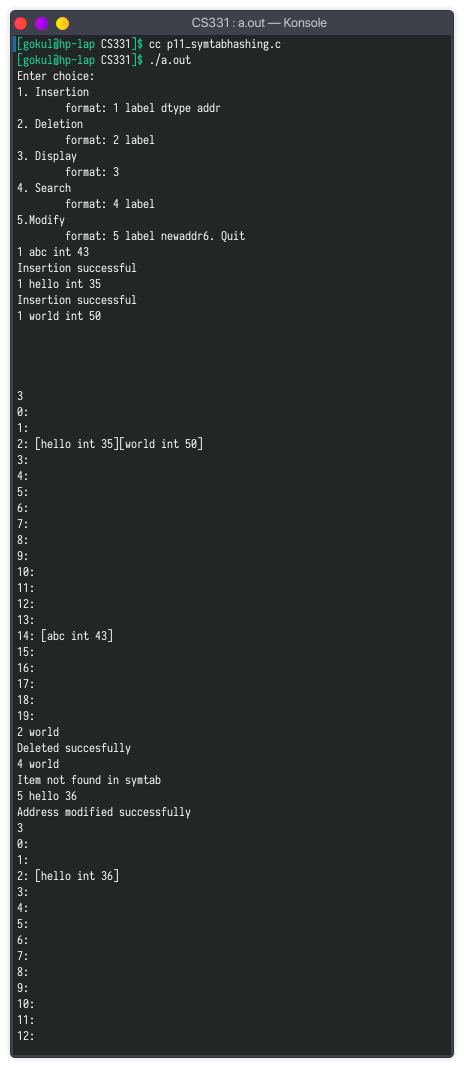
\includegraphics[]{img/p11.png}
    
\Large
\section*{Result}
\large
Symbol table with hashing is implemented and its output is verified
\end{document}